\documentclass{llncs}

\usepackage{epsfig}
\usepackage{color}

\renewcommand{\baselinestretch}{0.999}

%\setlength{\topmargin}{-0.5cm}
%\setlength{\oddsidemargin}{0.5cm}
%\setlength{\evensidemargin}{0.5cm}
%\setlength{\textwidth}{15.5cm}
%\setlength{\textheight}{22.5cm}

\newcommand{\todo}[1]
{\colorbox{yellow}{{\bf TODO:} #1}}

%\newcommand{\todo}[1]{}


\def\coaches{ {\bf COACHES}}

\begin{document}
%
%\frontmatter          % for the preliminaries
%
%\pagestyle{headings}  % switches on printing of running heads
%
%\mainmatter              % start of the contributions
%
\title{\coaches\\
Cooperative Autonomous Robots in Complex and Human Populated Environments}
%
%\titlerunning{SPQR}  % abbreviated title (for running head)
%                                     also used for the TOC unless
%                                     \toctitle is used
%
\author{L. Iocchi$^1$,  E. Erdem$^2$,  L. Jeanpierre$^3$, A.-I. Mouaddib$^3$, H. Sahli$^4$ \\
$^1$ Department of Computer, Control, and Management Engineering\\ 
Sapienza University of Rome, Italy\\
$^2$ ...
$^3$ ...
$^4$ ...
}

\institute{}
\date{}

%
%\authorrunning{L. Iocchi, D. Nardi, et al.}   % abbreviated author list (for running head)
%

\maketitle              % typeset the title of the contribution

\begin{abstract}

Public spaces in large cities are increasingly becoming complex, more hostile and  
unpleasant to use because of the overcrowding, rush and complex information in signboards. 
It is in the interest of cities to make their public spaces easier to use, friendlier to visitors and safer to increasing elderly population and to the people with disabilities. 
Meanwhile, we observe, in the last decade a tremendous progress in the development of robots in dynamic, complex and uncertain environments. The new challenge for the near future is to deploy the robots in public spaces to make easier and safer the use of these spaces. 

In this paper, we provide an overview of the COACHES project which addresses fundamental issues related to the design and development of autonomous robots with high-level skills for environment modeling and scene understanding, distributed autonomous decision-making, short-term interacting with humans and robust and safe navigation in overcrowding spaces. 
In particular, we describe the main components in which Artificial Intelligence techniques are used and integrated with the robotic system, as well as implementation details and some preliminary tests of these components. The implementation and the performed tests confirm the suitable integration of AI and robotics techniques to solve complex problems in complex environments, where human-robot interaction is a key feature.

\end{abstract}


\section{Introduction}
\label{sec:intro}

Public spaces in large cities are increasingly becoming complex and unwelcoming environments because of the overcrowding and complex information in signboards. It is in the interest of cities to make their public spaces easier to use, friendlier to visitors and safer to increasing elderly population and to the people with disabilities.
%
In the last decade, we observe tremendous progress in the development of robots in dynamic environments populated by people. There are thus big expectations in the deployment of robots in public areas (malls, touristic sites, parks, etc.) to offer services to welcome people in the environment and improve its usability by visitors, elderly or disabled people. 

Such application domains require robots with new capabilities leading to new scientific challenges: robots should assess the situation, estimate the needs of people, socially interact in a dynamic way and in a short time, with many people, the navigation should be safe and respects the social norms. These capabilities require new skills including robust and safe navigation, robust image and video processing, short-term human-robot interaction models, human need estimation techniques and distributed and scalable multi-agent planning.

\begin{figure}[t!]
\centering
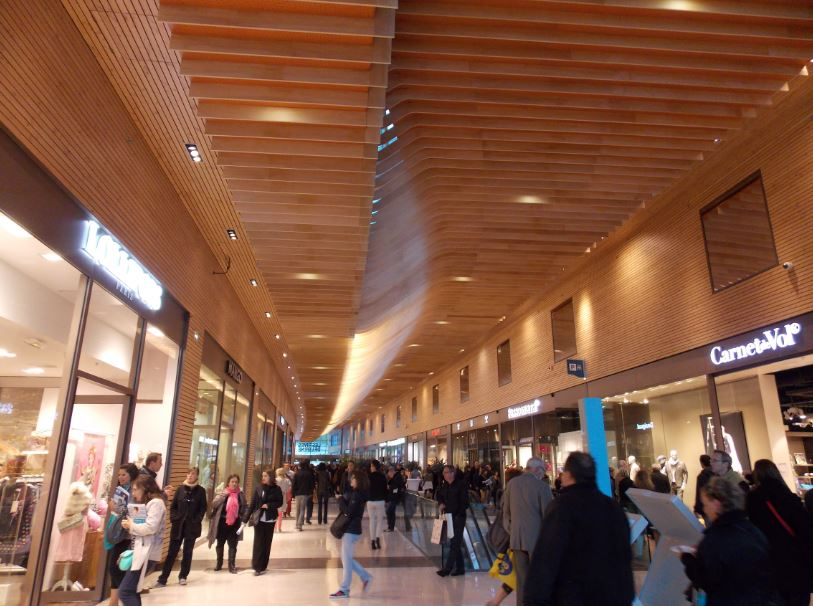
\includegraphics[width=0.65\textwidth]{fig/rivedelorne}
\hspace{0.8cm}
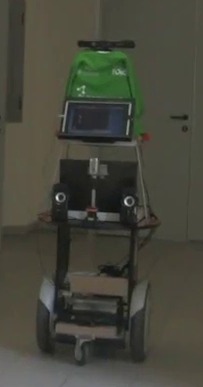
\includegraphics[width=0.255\textwidth]{fig/diago1}
\caption{\coaches environment and robot.}
\label{fig:env}
\end{figure}

The main goal of the \coaches project (October 2014 - September 2017)  is to develop robots that can suitable interact with users in a complex large public environment, like a shopping mall.
Figure \ref{fig:env} shows the \emph{Rive de l'orne} shooping mall in Caen (France) where the experimental activities of the project will be carried out, as well as a prototype of the robot that will be used.


Previous work on social robotics and human-robot interaction mostly focused on one-to-one human-robot interaction, including elderly assistance (e.g., GiraffPlus project \cite{CoCe14}) and interaction with children (e.g., MOnarCH project \cite{FeSe14}). Robots acting as museum tour-guides have also been successfully experimented. One of the first robot interacting with many non-expert users was RHINO deployed at the ``Deutsches Museum'' in Bonn,
Germany \cite{BuCr98}. In this work, the main focus was in the mapping, localization and navigation abilities in crowded environment, while human-robot interaction was limited to buttons on the robot, a remote Web interface and pre-recorded sentences issued by the robot.

As shown in the figure, in contrast with previous work, the \coaches environment is very challenging, because populated by many people.
Moreover, we aim at a more sophisticated interaction using multiple modalities (speech, gesture, touch user interfaces) and dialog generated on-line according to the current situation
and the robot's goals.
Consequently, the required level of ``intelligence'' of the \coaches robots in order to adequately perform complex and effective tasks in this environment in presence of people is much higher than in previous projects.

The proposed methodology to reach the project goals is based on integration of Artificial Intelligence and Robotics.
In this paper, we describe the main overall architecture of the system (Section 2) and the components related to Artificial Intelligence and Robotics (Section 3): 1) knowledge representation, 2) planning under uncertainty, 3) hierarchical plan execution and monitoring. 
Section 4 provides some examples and Section 5 concludes the paper.





\section{Software Architecture}

\begin{figure}
\centering
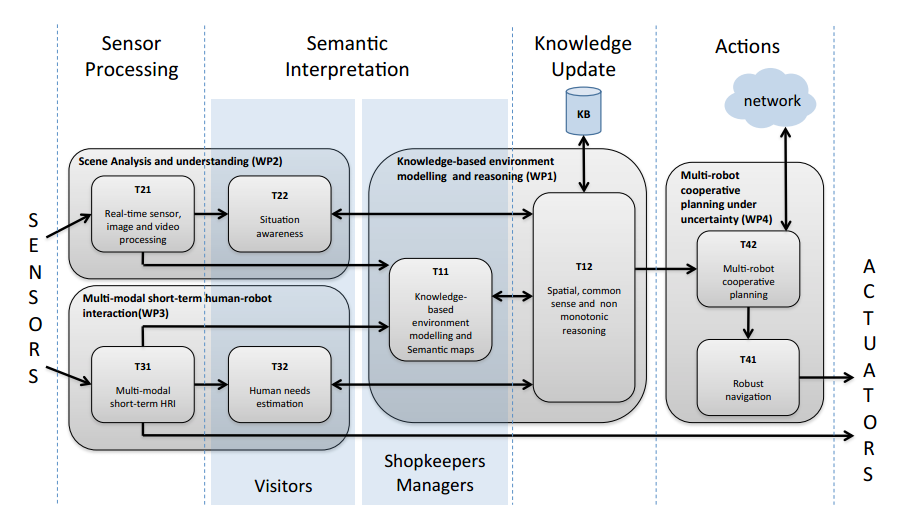
\includegraphics[width=0.9\textwidth]{fig/COACHES_swarch.png}
\caption{\coaches software architecture}
\label{fig:swarch}
\end{figure}

The software architecture of the \coaches robots is shown in Figure \ref{fig:swarch}).
An open architecture (hard/soft) and standard technologies available will be used, 
so that it will be easy to extend and/or adapt the capabilities of the system during the whole length of  the  project  (especially  to  integrate  and  test  various  algorithms  and/or  sensors).  
Such an open architecture will also simplify and optimize integration efficiency as well as re-use of assets in other projects or products. 


%For the development of the software robotics components, the Robot Operating System (ROS)\footnote{www.ros.org}, which is the standard middleware for robotics applications, has been selected.
%ROS provides the middleware infrastructure to effectively share information among the many modules implementing various functionalities on each robot. 
%Moreover, an interface (ROS-through-TCP) will be realized in order to share information among the robots and between ROS and non-ROS components of the system.

The main software components that will be developed for control, reasoning and interaction functionalities of the system are listed below.

\begin{itemize}
\item \emph{Scene analysis}, including sensor processing procedures for both on-board robot devices and static sensors in order to determine the current situation and understand events that are of interest for the system.

\item \emph{Multi-modal HRI}, defining a set of modalities for human-robot interaction, including speech recognition and synthesis, touch interaction, graphical interface on a screen mounted on the robot and Web interfaces.

\item \emph{Knowledge-based representation and reasoning}, defining the formalism and the procedure to represent and reason about the environment and the task of the robots.

\item \emph{Planning and execution monitoring}, for generating the plans to achieve the desired goals and monitor their execution for robust behaviors.

\item \emph{Safe navigation}, for guaranteeing safety operations of the robot in a populated environment.

\end{itemize}

%In the next section we will detail the components 
%\emph{Knowledge-based representation and reasoning} and
%\emph{Planning and execution monitoring},
%where Artificial Intelligence techniques have a fundamental role.





\section{Artificial Intelligence components}

While the overall software architecture described before integrates several components that are all important for the development of the project, in this paper we focus on the modules that implement a proper integration between Artificial Intelligence and Robotics techniques.
Thus, in this section, we will describe the three main components that allow the robots to: 1) represent and reason about the environment, 2) generate the plan to reach their goals; 3) monitor the execution to overcome failures.



\subsection{Knowledge base representation and reasoning}

%Knowledge based reasoning (semantic map, commonsense reasoning, ...)

The knowledge base (KB) is used to model both static knowledge (e.g., the semantic map of the environment and the common sense information) and the dynamic knowledge (e.g., human activities) coming from different units, such as the perception modules of the architecture, particularly the multi-modal HRI interface and the image processing modules. 
From these information, the reasoning module is able to infer the list of possible tasks to accomplish. This list of tasks is then sent to the decision module (described in the following section) that will compute the policy to accomplish them. 

Although there are many existing approaches to semantic representations of the environment (see \cite{KoGa14} for a survey), a standard formalism does not exist.
In this section, we thus define the main features of the knowledge base used in the project,
based on experience in previous work \cite{icar13bastianelli}. We first introduce the semantic labels used to describe elements of the world, then predicates that determine relations among these labels, and finally its application to the use case if the project.

\vspace{1em}

\noindent 
\textbf{Semantic labels}

In order to refer to objects and classes of objects in the knowledge base, we introduce a set of labels that will be associated to semantic meanings. 

A first set of these labels are called \emph{Concepts} and they are associated to classes of objects. For example, \emph{Restaurant} is a concept used in the semantic map to denote the class of restaurants in the shopping mall. Concept labels always start with an uppercase letter.
These concepts are organized in a hierarchical way according to the ``is-a'' relation.
In this way, we can express, for example, that the concept \emph{FrenchRestaurant} is a \emph{Restaurant}. 

A second set of labels will be used to denote objects. Each object belongs to a concept implementing the relation ``instance-of''. Object labels always start with a lowercase letter.
Thus, a particular restaurant in the mall will be denoted with an object label \emph{caf\'eMarcel} that will be instance of the concept \emph{FrenchRestaurant}. 

\vspace{1em}

\noindent 
\textbf{Predicates}

Predicates are used to describe relations among the semantic labels. For example, the ``is-a'' and the ``instance-of'' relations can be represented by the corresponding predicates {\tt\bf is-a} and {\tt\bf instance-of}. For example, we can write

\begin{quote}
{\tt\bf is-a}(FrenchRestaurant, Restaurant)\\
{\tt\bf instance-of}(caf\'eMarcel, FrenchRestaurant)\\
\end{quote}

%Sometimes,  the ``is-a'' and the ``instance-of'' relations will be abbreviated respectively by
%the operators $\subset$ and $\in$.
%Thus, the above example can also be described as \emph{FrenchRestaurant} $\subset$ \emph{Restaurant} and \emph{caf\'eMarcel} $\in$ \emph{FrenchRestaurant}.


Predicates are also used to denote properties of objects. For example, given the concepts \emph{Color} and \emph{Dress} and the objects \emph{red} $\in$ \emph{Color} and \emph{dress\_123} $\in$ \emph{Dress}, the predicate 

\begin{quote}
{\tt\bf color}(dress\_123,  red)
\end{quote}

\noindent
will represent the color property \emph{red} of the particular object  \emph{dress\_123}.




\vspace{1em}

\noindent 
\textbf{Example of representation of the environment}

For representing the \emph{Rive de l'orne} shopping mall, we consider different types of areas: shops, restaurants, halls, corridors, rest areas, offices, toilettes, etc. For shops, services and restaurants we consider different categories:
\begin{itemize}
\item {\it Shop categories}: dress shop , women dress shop, kid dress shop, men dress shop, makeup store, store perfume, sport store, etc.
\item {\it Restaurant categories}: French, Japanese, Chinese, Italian, Oriental, African, fast-food, etc.
\item {\it Service categories}: security, information, health-care, etc.
\end{itemize}

All these areas are represented as concepts that are grouped in a more general concept \emph{Area}. The hierarchy of these areas will be defined through the ``is-a'' relation of the semantic labels described before.

Doors are also considered as connections of these areas. \emph{Door} is a concept containing door objects and connections of areas through doors are represented with the {\tt\bf connect} predicate (see also below).

\begin{quote}
{\tt\bf connect}(door12, area1, area2)
\end{quote}

\noindent
where \emph{door12} $\in$ \emph{Door} \emph{area1}, \emph{area2} $\in$ \emph{Area}  are objects belonging to the corresponding concepts. Moreover, the status of the door can be expressed with a predicate {\tt\bf open}. For example,

\begin{quote}
{\tt\bf open}(door12) \\
\end{quote}


%\vspace{1em}

\noindent 
\textbf{Reasoning} 


The KB is used by reasoning procedures that will be implemented in order to reason about the current situation and to define a set of goals that the \coaches robots have to achieve.
To this end, the reasoning engine takes into account the available information in the KB related to: semantic map, common-sense knowledge and dynamic knowledge coming from the Scene analysis module and determine which goals for the system are consistent with the current situation. This set of goals is then passed to the Planning module described below.



\subsection{Planning under uncertainty}

In this section we describe the Markov Decision Process (MDP) used to model the \coaches planning domain and the algorithm implemented for computing the optimal policy.

\vspace{1em}
\noindent
{\bf Task structure}

The result of the reasoning module (KB module) is a set of goals $G = \{ g_{1}, g_{2}, \ldots, g_{k} \}$ concerning advertisement, patrolling, assisting and escorting.  We note also that advertising goals could be performed in parallel with the moving ones.  Consequently, the task structure is a hierarchy of modules to execute. This structure is  inspired by progressive processing units \cite{CarMouIjcai01}, that we  name PRU+. In our application, we define four PRU+. Each PRU+ is composed of levels where the first level concerns the execution of the subtask {\sc goto site $X$}, the second level concerns the advertisement at a location $(x,y)$ and the third level consists of {\sc do task $X$} where $X$ could be  the assistance, the patrolling, the escorting or the surveillance.% (see Figure \ref{FigureEscortTask}). 
With such task structures we can also define some joint goals requiring joint PRU+.  For example, escorting a people from one location in a building to another location in the other building requires a cooperation between robots. Indeed, the first robot executes a policy of PRU+ for escorting a user to the exit of the first building, provide him/her information to reach the other building and then send information to the other robots in the other building to continue the escorting task at the second building. The structure of tasks we propose for single robot tasks is  {\sc \{goto $x$, advertisement, do $x$\}}, while for the joint task is {\sc \{goto $x$, advertisement, inform people, send message to the other robots\}}. 
The task {\sc do $x$} concerns different tasks of assistance. 

More formally, a PRU+ is defined by a set of levels $\{ l_{1}, l_{2}, \ldots, l_{k} \}$, where each level $l_i$ is composed by a set of modules $\{m_{i}^{1}, m_{i}^{2}, \ldots, m_{i}^{p_{i}} \}$ and each module $m_i^j$ is defined by different execution outcomes that we name options $\{ \alpha_{i}^{j}, \beta_{i}^{j}, \ldots \}$.  From these elements, a PRU+ language is defined allowing to define tasks as PRU+ as given in the following example.  

\vspace{-1em}
\begin{small}
\begin{verbatim}
<pru>
  <Start>
    <SVU>
      location := RobotPos
      desire := nil
    </SVU>
    <Next> 
      1.advertise 
      1.advertiseComplex 
      1.interact
    </Next>
  </Start>
  <Layer id='1'>
    <StateVariable id='location' />
    <StateVariable id='desire' />
    <Action id='advertise'>
      <Parameter id='X' domain='AvailableAds' />
      <Outcome id='done' p='1.0'>
      <Quality kind='null' const='100' />
      <Duration kind='distance' const='3' />
      <SVU> location := $X </SVU>
      <Next> 
        1.advertise 
        1.advertiseComplex 
        1.interact
      </Next>
      </Outcome>
    </Action>
    <Action id='advertiseComplex'>
    ...
</pru>
\end{verbatim}
\end{small}

\vspace{1em}
\noindent
{\bf MDP definition and planning}

The planning procedure consists of formalizing the robot activities as an MDP using the PRU+ task definition. This procedure is based on two steps: 1) generating an MDP from a PRU+, 2) compute the optimal policy for the generated MDP.
In the following we define the $MDP = <S, A, R, T> $ where : 
\begin{itemize}
\item $S$ is a set of states defined by $[l, m, o, SVU]$ where $l$ is the level of the PRU, $m$ is a module of the level $l$, $o$ is an option of module $m$ and SVU are  state variables defining the execution context representing the subset of variables to be considered for the option $o$. 
\item $A$ is the set of actions consisting of execution of one module of the next levels $E$ or skipping the level  $S$. 
\item T is the transition function defined as follows : 
\begin{itemize}
\item $ Pr([l+1,m',o',svu'] | [l,m,o,svu], E) = p(o')$, this means when execution module $m'$ at state [$l,m,o,svu]$ we move to state $[l',m',o',svu']$ with probability p(o') representing the probability to get the outcome $o'$. % (for example executing module goto location (4,5), there is a probability p((3,5)) to get the outcome (3,5) because of uncertainty.
\item $Pr([l+2, m' , o' , svu' ] | [l,m,o,svu], S) = 1$, this transition is deterministic because we skip level $l+1$ and we move to level $l+2$. 
\end{itemize}
\item R is the reward function related to the options assessing the benefit to get the outcome; 
\end{itemize}

From this definition the Bellman equation of our former, becomes : 
\[ V([l,m,o,svu]) = R(o) + max_{E,S} \sum Pr([l',m',o',svu'] | [l,m,o,svu], a). V([l',m',o',svu'] )  \]

The optimal policy $\pi$ is computed by a standard MDP solving algorithm based on value-iteration. Moreover, in this algorithm, a tabu-list of actions is used to choose or drop actions to be inserted in the policy.
This tabu-list is built and updated by the Model updater module, described below in this section, representing the actual feedback coming from the execution layer.



\subsection{Plan execution and monitoring}


Plan execution monitoring and interleaving planning and execution are crucial features for an autonomous robot acting in a real environment, specially when human interaction is involved, 
as for the \coaches robots. Indeed, in complex scenarios, it is not possible to model and foresee all the possible situations that may occur, consequently plans generated off-line (i.e., before the actual execution of the task), when several information about the real environment are not known, may not be optimal or feasible at execution time.

It is thus necessary to explicitly model and consider possible plan failures and to devise a mechanism that is able to properly react to these failures. Moreover, on-line replanning (i.e., planning after plan failures) may not be feasible when the model itself is inaccurate, since the same cause of the plan failure (typically a non-modeled feature of the environment) will likely occur also in next executions.

To this end, we have defined a plan execution and monitoring framework composed by three modules: a planner (as described in the previous section), an executor, and a model updater. The three modules cooperate during the execution of a complex task for a robot and provide for a feedback mechanism from execution to planning.
More specifically, the following interactions are devised:
1) the planner notifies on-line to the executor the best plan (policy) to be executed according to the current model of the world; 2) the executor executes this plan (policy) and determines success or failures of the actions; 3) each failure is reported to the model updater that will follow some rules (either automatic domain dependent or manual domain dependent) to modify the current model, so that the planner can generate a new plan that is more suitable for the current situation as detected by the executor.

The execution module is based on the Petri Net Plan (PNP) formalism\footnote{pnp.dis.uniroma1.it} \cite{ZiIo11PNP}. 
PNP is a formalism to represent high-level plans for robot and multi-robot systems. Being based on Petri Nets, it is very expressive and can thus represent durative ordinary and sensing actions, and many constructs such as sequence, loop, interrupt, fork/join, and several multi-robot synchronization operators.
PNPs are used to model the behavior (i.e., the policy) that is generated by the planner module and to execute it using the PNP-ROS implementation that allows ROS actions to be executed under the control of a PNP.


The two main components of this process will be described in the rest of this section:
1) Policy to PNP transformation; 2) Model updater.

\vspace{1em}
\noindent
{\bf Policy to PNP transformation}

The policy generated by the MDP planner is automatically transformed in a PNP.
For this process, the MDP planner produces the following information: the initial state,
one or more goal states, state-action pairs implementing the policy and the conditions to
be checked when non-deterministic actions are executed. 
States, actions and conditions are represented just as unique labels.
With this input, the algorithm for generating the corresponding PNP is based on a recursive procedure for building the graph corresponding to the policy, starting from the initial state to the goal states, applying the state-action pairs for each state and adding a sensing operator for every non-deterministic effect of an action.

The labels in the policy and in the PNP referring to actions correspond to implemented actions, according to the ROS actionlib\footnote{http://wiki.ros.org/actionlib} notation,
while labels referring to conditions correspond to sensor processing procedures that
evaluate their truth based on the current information available to the system.

The PNP generated with this process does not contain a representation of action failures.
This is obtained by defining a set of execution conditions for each action and by automatically adding action interrupts when these conditions are not valid. In this way the new PNP will be able to actually check execution conditions of actions and to interrupt the plan is these conditions are not valid. For example, an execution condition of a communication action is that a person is in front of the robot. While executing the action, the condition of a person being in front of the robot is checked and, if it becomes false, the action is interrupted.

When an interrupt is activated, the flow of execution of the plan can follow one of the two following lines: 1) \emph{internal recovery procedure}\footnote{At this moment, the \emph{internal recovery procedures} are manually written, while some automatic technique could be devised.}, when the current plan itself contains a recovery behavior (i.e., a sub-plan or portion of the plan) for dealing with this failure; 2) \emph{plan failure}, when the current plan is not able to deal with this kind of failure.

In the latter case, the executor sends to the Model updater module the following information:
1) action failed, 2) condition that was checked to determine action failure, 3) status of the plan (that can contain additional conditions useful for diagnosis of the failure).
Given this input, the Model updater module (described in the next paragraph) modifies the MDP model of the domain and activates a new planning procedure to generate a new plan (policy) that aims at avoiding at least the failure cause just occurred.

\vspace{1em}

\noindent
{\bf Model update}

The problem of updating a planning model, given the feedback of the execution of the plan, is very relevant for actual application of planning techniques to real problems, but, to the best of our knowledge, this problem has not been investigated explicitly and a general solution does not exists.

At this moment, we have implemented a simple method that build and maintains a tabu list of actions to be selected in the MDP planning process.
More specifically, whenever an action fails, the action is inserted in the tabu list and thus it will not be selected in the next generation of the policy.
This mechanism is also tied to a time decay mechanism, so that the presence of an action in the tabu list decreases over time, making the action available some time after the action failed, in order to try it again in the future.

For example, if the action of moving to a particular shop fails because there are too many people in that area, the robot will avoid to generate a new plan that will include going to that shop for a while, avoiding thus the main cause of the current failure.

Although not optimal, this strategy allows the robot to generate new plans after failures that will not determine the same cause of failure with respect to the one just failed. 








\section{Implementation and tests}

\todo{The COACHES robots are under construction, so we use a simulator...}





\subsection{Simulator environment}

The simulation environment is based on 2D Stage simulator, that is integrated in the ROS infrastructure. The choice of a 2D simulator (instead of a 3D one) is motivated by: 1) the need of modeling and testing high-level behaviors of the robot that does not involve 3D perception, 2) the possibility of using the simulator for multiple robots and other moving elements representing people in the environment, 3) the possibility of using the simulator on standard laptop, thus not requiring advanced graphical cards for running 3D simulations.

\begin{figure}
\centering
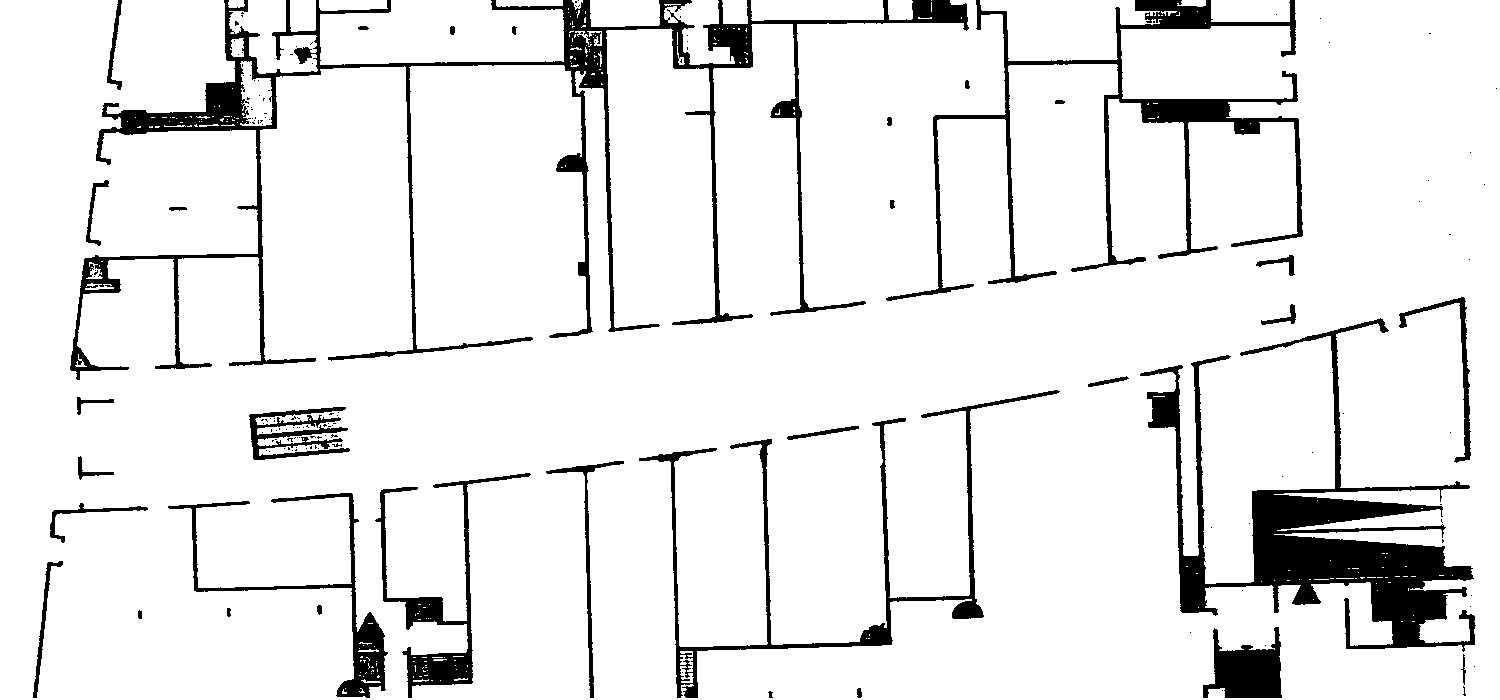
\includegraphics[width=0.95\textwidth]{fig/Rive1.png}
\caption{2D map of the \emph{Rive de l'orne} shopping center.}
\label{fig:stage}
\end{figure}


In the Stage simulator the following map of the \emph{Rive de l'orne} shopping center has been realized. In Figure \ref{fig:stage} a section of the shopping mall in which we will deploy the prototypes is shown.
Additional maps have been realized for reproducing the environments of the partners in which some experiments will be performed.

The Stage environment models one or more robots that have the same 2D sensor and actuator configurations as the real ones and some additional mobile obstacles that represent people moving in the environment. Several behaviors can be tested in this simulated environment such as: 2D perception of human behaviors, human-robot social navigation (e.g., following a person or guiding a person), safe navigation in the environment.

The Stage environment has been fully realized and tested and this configuration will be used as a reference also for the development of the real robotic system.

\subsection{Plan generation and execution tests}

The following tests have been performed in the simulator to verify the suitability of the proposed software architecture and of its components. In particular, we have used the simulated environment to assess the suitability of the AI components described in the previous section.

\begin{itemize}
\item Simple Move-To behavior: moving the robot from one place to another allows for testing the map description, path planning, and the global architecture.
\item Patrol behavior: moving the robot across several places allows for testing the sequential decision-making, along with the dynamic addition of new places to visit or new obstacles.
\item Simple interaction: going to some people for initiating an interaction allows for testing the difficulties introduced by non-stationary goals, along with the dialog system. It also makes it easier to test for branching behaviors since the dialogs may have several different outcomes.
\end{itemize}

\todo{Describe some runs in simulation}




\section*{Acknowledgements}

\coaches ~ is funded within the CHIST-ERA program ...

\begin{small}
\bibliographystyle{plain}
\bibliography{bib/inc-short,bib/2000-2004,bib/2005-2009,bib/2010-2014}
\end{small}


\end{document}

